\section{Problemstilling}
Reinseanlegget er teknisk utdatert og treng modernisering. Styringssystemet, som no er over tjue år gammalt,
består hovudsakeleg av eldre og utgåtte komponentar. Med eldre komponentar aukar risikoen for svikt, 
og det kan vere vanskeleg å finne passande reservedelar.

WaterCare, som opphavleg leverte styresystemet, har i seinare tid blitt avvikla. Dette gjer at kompetansen 
og moglegheita for å gjere endringar i styresystemet er vanskeleg. 
På grunn av desse utfordringane har ikkje anlegget klart å halde tritt med den teknologiske utviklinga, 
og mindre problem har gradvis bygd seg opp til større utfordringar.

Samstundes med desse faktorane er dokumentasjonen til reinseanlegget mangelfull, noko som gjer at enkle arbeidsoppgåver blir utfordrande og tidkrevjande.
I verste fall kan styresystemet til anlegget svikte. Med dei ovanfor nemnte utfordringane vil det være krevjande
å få anlegget i drift igjen. Dette representera eit kritisk problem innan avlaupshandtering og kan ikkje oversjåast.
\newline



%\begin{figure}[htbp]
%    \centering
%    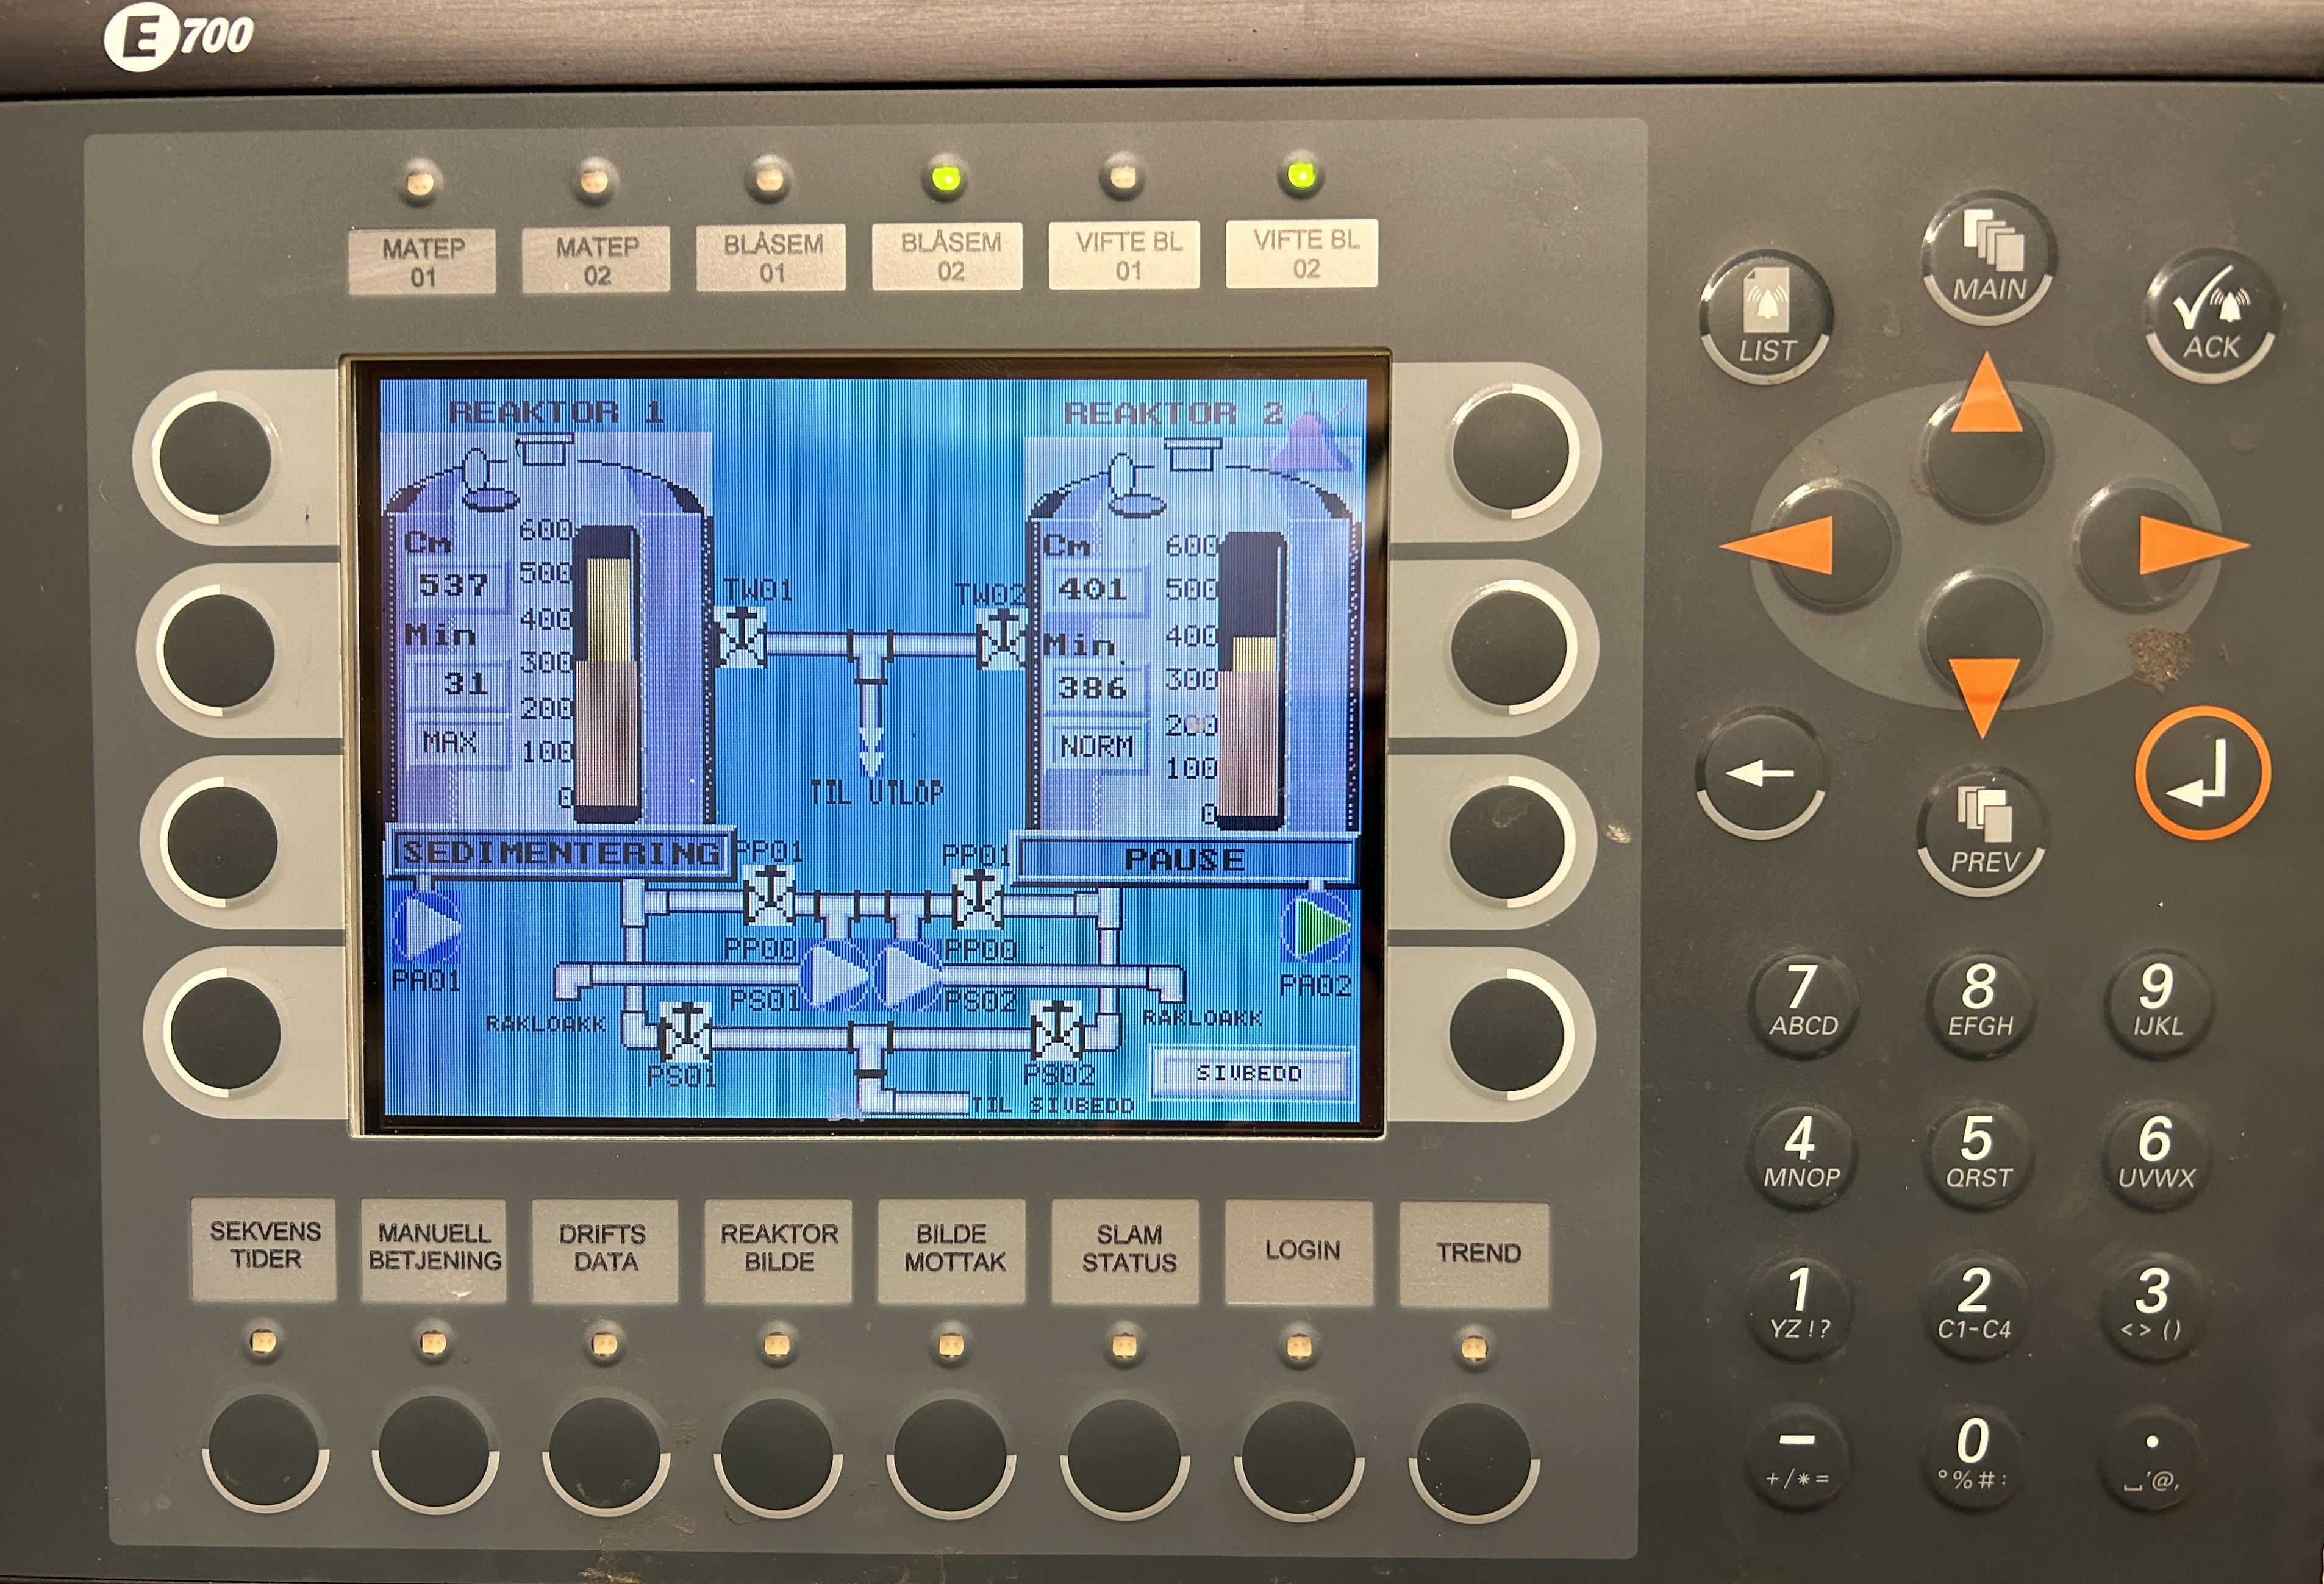
\includegraphics[width=0.8\textwidth]{Bilder/BeijerSkjerm.JPG}
%    \caption{Beijer HMI}\label{fig:HMI}
%\end{figure}


\begin{figure}[htbp]
    \centering
    \begin{subfigure}[b]{0.5\textwidth}
        \centering
        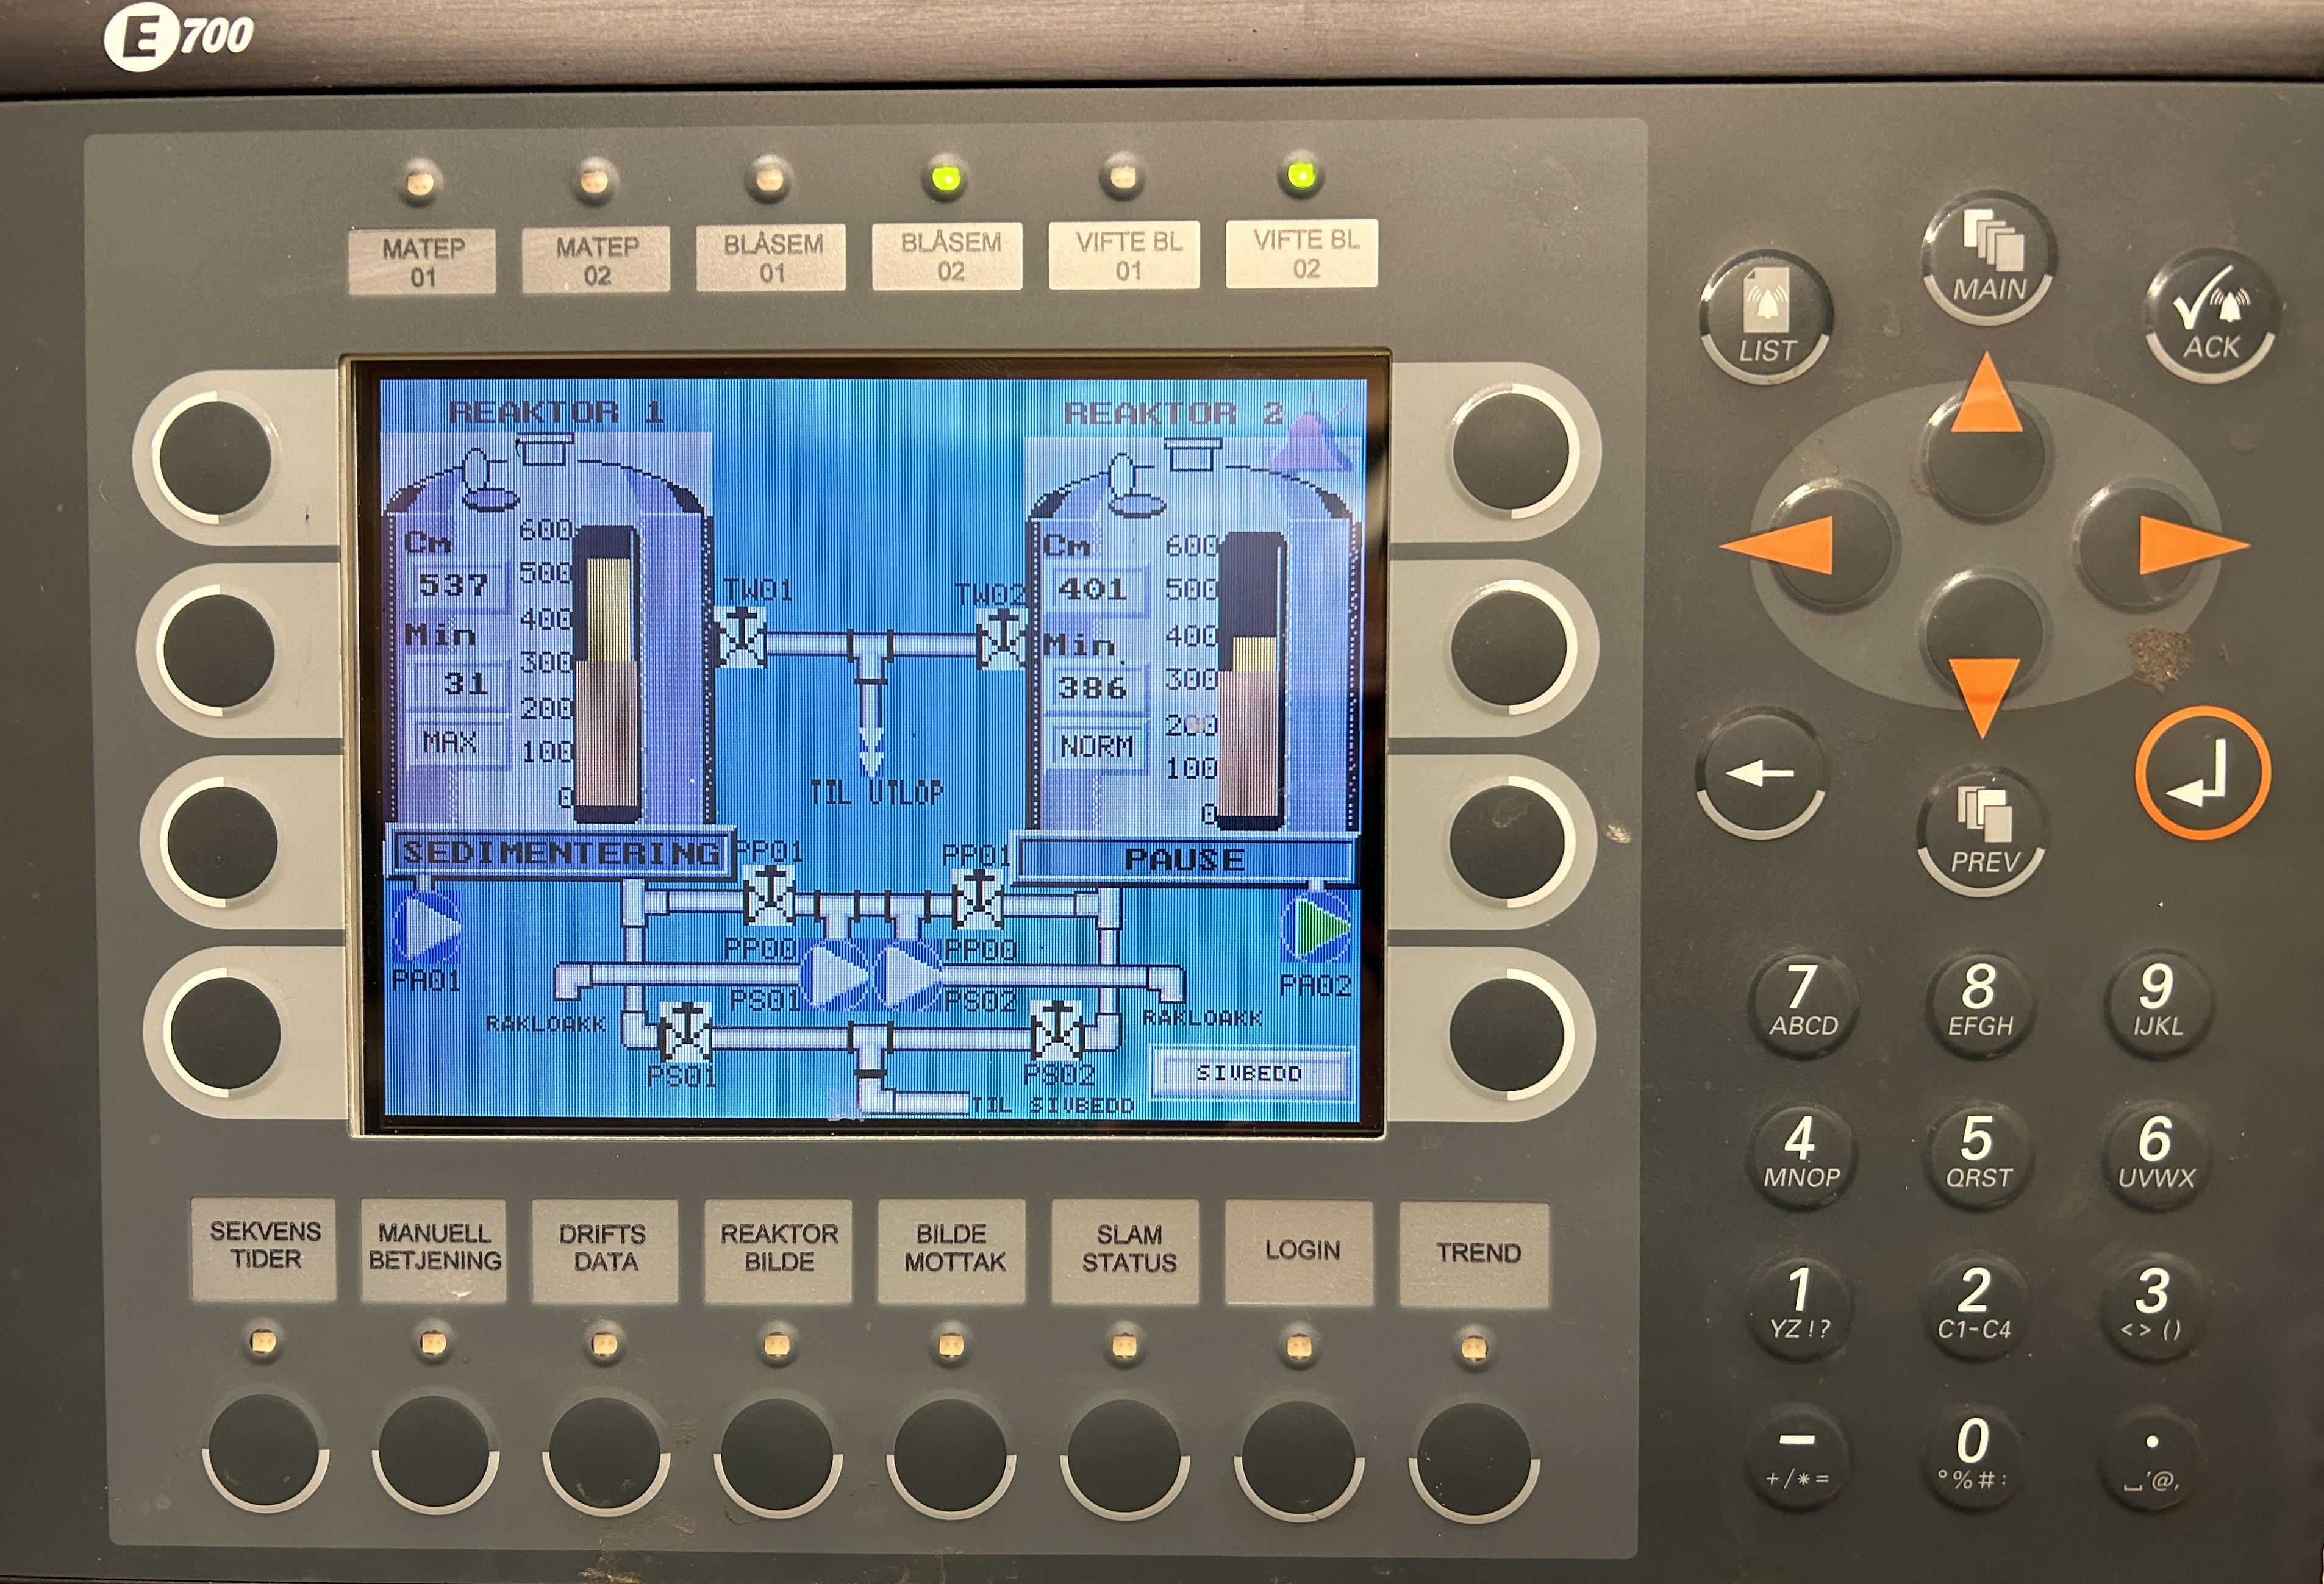
\includegraphics[width=1\textwidth]{Bilder/BeijerSkjerm.JPG}
        \caption{Beijer HMI}\label{fig:subfig1}
    \end{subfigure}
    \hfill
    \begin{subfigure}[b]{0.3\textwidth}
        \centering
        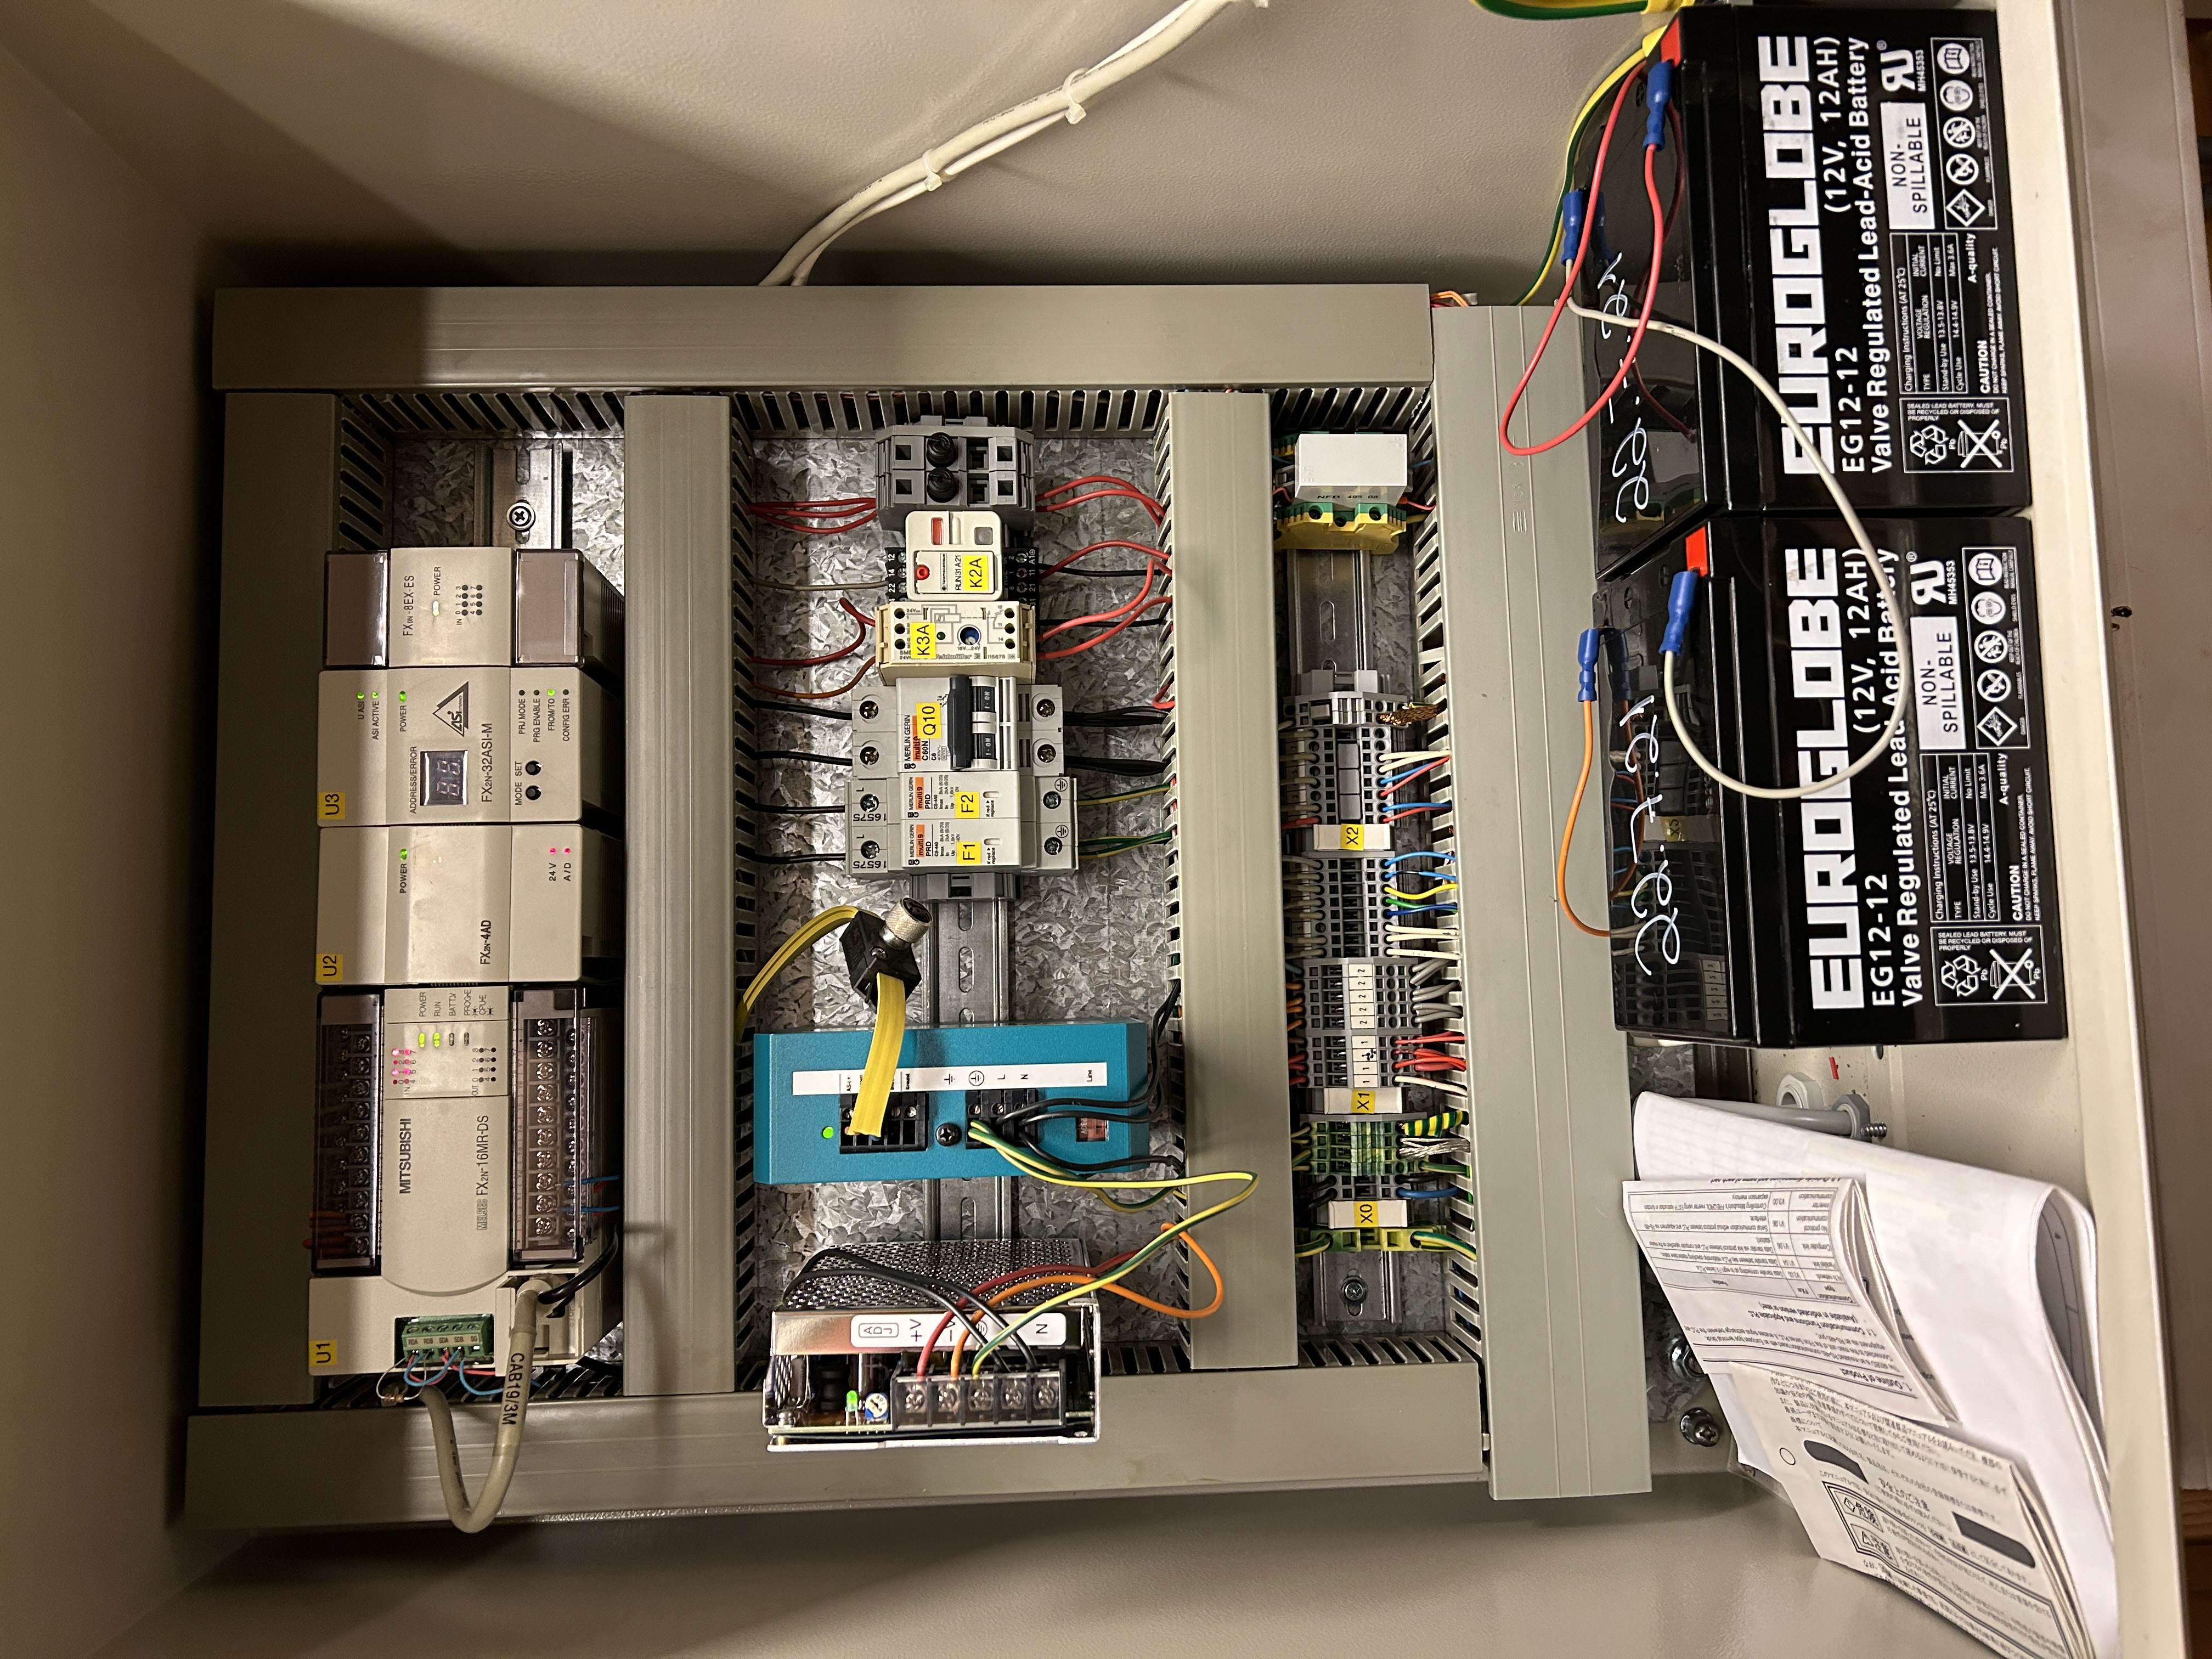
\includegraphics[angle=-90,width=1\textwidth]{Bilder/Styreskap.JPG}
        \caption{Styreskap}\label{fig:subfig2}
    \end{subfigure}
    \caption{Styresystem}\label{fig:Styresystem}
\end{figure}